\documentclass[10pt]{article}
\usepackage{parskip}
\usepackage[utf8]{inputenc}
\usepackage[left=2.00cm, right=2.00cm, top=2.00cm, bottom=2.00cm]{geometry}
\usepackage[spanish]{babel}
\usepackage{graphicx,subfig}
\usepackage{fancyhdr}
\graphicspath{{Imagenes/}}
\usepackage{enumerate} 
\usepackage{multicol}
\usepackage{tabularx}
\usepackage{hyperref}
\usepackage{amssymb}
\usepackage{adjustbox}
\usepackage{amsmath}
\usepackage{cancel}
\usepackage{url}
\usepackage[usernames]{color}
\begin{document}


\pagestyle{fancy}
\cfoot{}


%Cabeceras
\rhead{Infografia}
\lhead{}

%Portada
\begin{titlepage}
	\newgeometry{
		left=25mm,
		right=25mm,
		top=5mm,
		bottom=30mm,
		headheight = 0 mm
	}

	\begin{figure}[t]
		\subfloat{
\includegraphics[width=0.15\textwidth]{Logo_IPN}}
		\hspace{0.6\textwidth}
		\subfloat{
\includegraphics[width=0.22\textwidth]{LogoEsime}}
	\end{figure}

	\centering
	{\bfseries\Huge Instituto Politécnico Nacional. \par}
	\vspace{1cm}
	{\scshape\Large Ingeniería en Comunicaciones y Electrónica. \par}
	\vspace{0.3cm}
	{\scshape\Large Laboratorio de Electricidad y Magnetismo.  \par}
	\vspace{1cm}
	{\scshape\Huge Victoria la Reina Insaciable \par}
	\vspace{1cm}
	{\itshape\Large Ley de Ohm. \par}
	{\Large 2CM13\par}
	\vfill
	{\Large Autores: \par}
	{\Large José Emilio Hernández Huerta. \par}
	{\Large Nataly Bejarano Garduño.\par}
	\vfill
	{\Large Junio 2023. \par}

\end{titlepage}

\newpage

\section{Resumen.}
Esta es una pequeña investigación en la cual se aglomeran los conceptos sobre; la ley de inducción de Faraday, la ley de Ampere, la ley biot-savart y la ley de Lenzt

\begin{multicols}{2}

\section{LEY DE INDUCCIÓN DE FARADAY}
Si se tiene una bobina conectada a un instrumento
capaz de medir diferencia de potencial eléctrico,
puede verificarse que al acercar o alejar un imán a
una de las entradas de la bobina puede medirse un
"voltaje" (si el medidor es suficientemente sensible y
capaz de medir variaciones rápidas), que llamamos
''fuerza electromotriz (fem) inducida ''($\varepsilon$) a través de
los terminales de la bobina.
Los resultados experimentales indican que es útil
definir (como se ha hecho con el campo
electrostático) el flujo de campo magnético: \\
\begin{center}
	$ \phi_{B} = B_{\perp} \cdot A = B \cdot A_{\perp} = B \cdot A \cdot cos(\varphi) $\\
\end{center}

"Las unidades del flujo son tesla. metro cuadrado, llamada ''weber'' (Wb) para honrar a Whilhelm Weber, uno de
los primeros investigadores del magnetismo: 1 Wb = 1 T.m2
. ..."
"Los resultados de las observaciones anteriores, para una espira de alambre, se pueden escribir con: \\
\begin{center}
	$\varepsilon - \frac{\nabla \phi_{B}}{\nabla t}$

\end{center}
de la cual explicaremos el significado del signo de menos más adelante. Una sola espira de alambre desarrollará un
voltaje inducido (en volts) que es igual a la rapidez de cambio del flujo magnético que la atraviesa, con respecto al
tiempo, en cualquier instante dado (en unidades SI, la constante de proporcionalidad es 1). Si hay N vueltas de
alambre en una bobina, cada una tiene un voltaje inducido que está en serie con las demás, de tal forma que la
fem inducida promedio es \\
\begin{center}
	$\varepsilon = -N \cdot \frac{\nabla \phi_{B}}{\nabla t} $
\end{center}
que es una de las ecuaciones fundamentales del electromagnetismo. Es un resumen de observaciones, y no se
puede deducir a partir de fórmulas anteriores. Por lo general se llama ley de inducción de Faraday a esta
ecuación, aunque Faraday nunca la escribió. "
\href{https://www.youtube.com/watch?v=B6V9AAlcChE}\textcolor{blue}{Inducción}}
%------------------------------------------------
\section{LEY DE AMPERE}
La ley de Ampère determina que la circulación del campo magnético a lo largo de una línea cerrada es equivalente a la suma algebraica de las intensidades de la corrientes que atraviesan la superficie delimitada por la línea cerrada, multiplicada por la permitividad del medio. En concreto para el vacío:\\
\begin{center}
	$\oint \vec{B} \cdot \vec{dl} = \mu_{0} \cdot \sum I $ 
\end{center}

\href{https://www.youtube.com/watch?v=tqw9xw_20Qk}{\textcolor{blue}{Video Ampere}}
\subsection{El electroimán}
Ejemplo de aplicación de la ley de Ampère: el electroimán. Un electroimán es un tipo de imán que se activa cuando circula una corriente eléctrica por él. Habitualmente, los electroimanes estan formados por un gran número de espiras de alambre muy próximas entre sí.
Si los extremos de este alambre estan conectados a una diferencia de potencial, circula la corriente eléctria por él y se genera un campo magnético.
Este campo magnética es equivalente a la suma de los campos magnéticos de cada espira y se puede calcular aplicando la ley de Ampère.


\section{Ley de Biot-Savart}
El campo magnético creado en un punto próximo (p) a un conductor por el que circula una corriente
I, es proporcional a la intensidad de la misma, a la permeabilidad ($\mu$) del medio e inversamente
proporcional a la distancia al cuadrado a dicho conductor.
La permeabilidad ($\mu$) es equivalente a la permitividad ($\varepsilon $) del campo eléctrico pero; se encuentra
en el numerador, es decir, a mayor µ mayor campo. Esta variable está tabulada, según el material
(medio), y me dirá cuanto aumenta el campo B según donde está el conductor con corriente (la
bobina).
Realizando algunos cambios de variables (ver PDF facultad Rosario) se determina que en un punto
próximo de un conductor muy largo (o punto cercano al mismo respecto al largo) el campo B es:

\begin{center}
	$ B = \frac{\mu_{0}}{2\pi R} $
\end{center}
a la distancia perpendicular del conductor al punto considerado.
$\mu$0 es la permeabilidad del vacío, muy próxima a la del aire 4$\pi$ 10-7
Tesla metro /Ampere.
Recordando que la Tesla es N/A m queda también $\mu$0= 4$\pi$ 10-7 N /A2
.
(Recordar que el campo E producido por una carga q es E= q / 4$\pi \epsilon$0 r
2
donde r es la distancia a la
carga q)

\begin{center}
	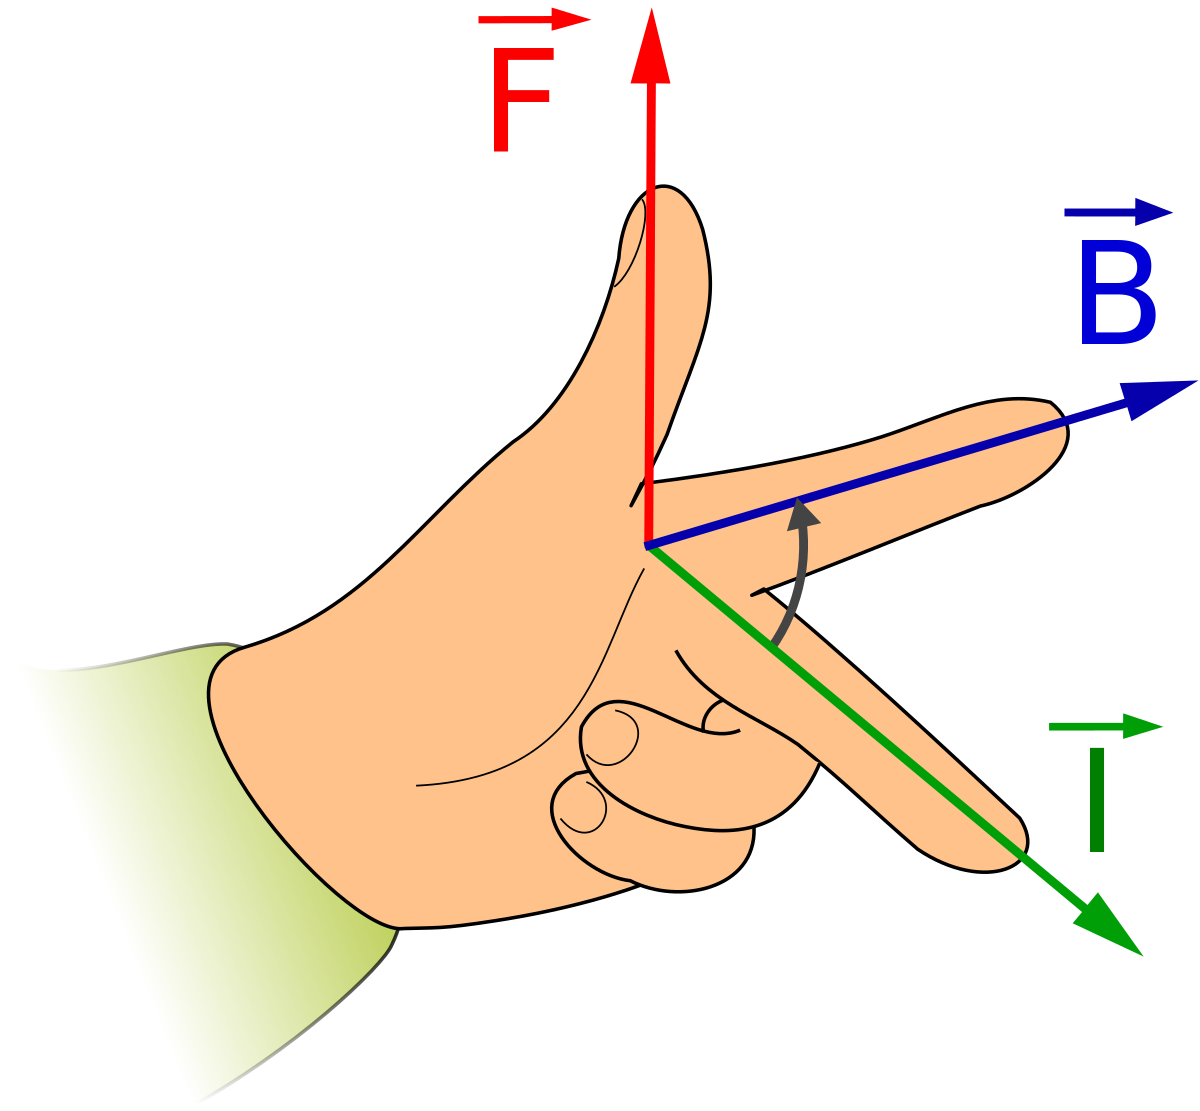
\includegraphics[width=0.3\textwidth]{Imagenes/ManoLaplace.png}
\end{center}
\href{https://www.youtube.com/watch?v=WSDVvHvIEk4}{\textcolor{blue}{Ley de Biot-Savart}} 
\subsection{LEY DE LENZ}
La ley de Lenz establece que al generar una fuerza electromotriz (fem) provocada por una cambio del flujo magnético según la ley de Faraday, la polaridad de fem inducida genera una corriente magnética que se opone a la variación que produce.

Esta ley se basa en la ley de inducción de Faraday que establece que cuando se conecta un campo magnético variable a una bobina, se induce una fuerza electromotriz (voltaje inducido) en él. Dicho de otra forma: la magnitud de la fuerza electromotriz inducida en el circuito es proporcional a la variación del cambio de flujo.

La ley es una consecuencia al principio de conservación de la energía (la energía no se puede crear ni destruir) y a la tercera ley de Newton (siempre hay una reacción igual y de sentido contrario a cada acción).


\begin{center}
	$ \phi = B \cdot S \cdot \cos{a}$
\end{center}
donde

$ \phi$ es el flujo magnético expresado en Wb.
$B$ es la inducción magnética expresada en T.
$S$ es la superficie plana del conductor.
$ \alpha $ es el ángulo formado por la dirección del campo y la superficie del conductor.
\href{https://www.youtube.com/watch?v=Grgiuwo4bUY}{\textcolor{blue}{Lenz}} 
\href{https://www.youtube.com/watch?v=ywlsOYtDXHE}{\textcolor{blue}{Lenz}} 




\end{multicols}

\end{document}
